\chapter{Umsetzung}

Bei der Umsetzung ist die erste Frage, die zu klären ist, mit welcher Programmiersprache gearbeitet werden soll.
In diesem habe ich mich aus verschiedenen Gründen für \textit{Python} entschieden.
Der erste ist, dass \textit{Python} bereits im Masterprojekt verwendet wurde und so die Integration leichter fällt.
Als zweites geht es speziell um die Bibliothek \textit{PySpark}.
\textit{PySpark} ist die Bibliothek, mit deren Hilfe \textit{Apache Spark} in \textit{Python} verwendet werden kann.
Neben \textit{PySpark} gibt es auch Bibliotheken für die Sprachen \textit{Java} und \textit{Scala}.
Der entscheidende Unterschied hierbei ist aber, dass \textit{Python} eine interpretierte Sprache ist.
Das bedeutet, dass der geschrieben Programmcode nicht in Maschinensprache übersetzt wird, sondern durch einen sogenannten Interpreter ausgeführt.
In diesem Anwendungsfall hat das den Vorteil, dass die Spark-Jobs nicht als kompilierte jar-Datei explizit ausgeführt werden müssen, sondern der Interpreter sich an den entsprechenden Zeitpunkten um die Ausführung kümmert.
Das bedeutet, dass die Konfiguration eines Spark-Jobs dynamisch während der Ausführung des Programms gemacht werden kann und man so mehr Freiheit für die Entwicklung bekommt.
Der letzte Vorteil ist, dass Programmcode dynamisch aus Dateien nachgeladen werden kann, was für die Umsetzung der Plugins wichtig ist.

\section{Voraussetzungen}
Um das Datalake System umsetzen zu können müssen einige Voraussetzungen erfüllt sein.
Die erste ist, wie in \ref{fig:ingestion_arch} bereits beschrieben, dass ein Server benötigt wird, der sich um die Verteilung von Nachrichten kümmert.
Als zweites muss außerdem ein zentraler Speicher für Dateien bereit stehen, indem sowohl Datenquelldateien als auch Plugindateien abgelet und von jedem Server abgerufen werden können.

\subsection{Apache Kafka}

\textit{Apache Kafka} ist ein verteiltes Event-Streaming-System, dass nach dem Publish-Subscribe-Muster funktioniert.
Events können von Produzenten in das System veröffentlicht werden und Konsumenten können diese Events abonnieren.
Das ganze läuft dabei in Echtzeit ab.
Durch seine Verteilung kann \textit{Kafka} den Ausfall einzelner Server ausgleichen.
Außerdem können Ströme von Events für einen beliebigen Zeitraum abgespeichert werden.

\textit{Kafka} besteht aus einem Cluster von Servern und verschiedenen Clients.
Es gibt zwei Arten von Servern.
Einige bilde die Speicherebene von \textit{Kafka} und werden Broaker genannt.
Die anderen verwenden \textbf{Kafka Connect}\footnote{https://kafka.apache.org/documentation/\#connect} um extierende Systeme, zum Beipsiel eine Datenbank, in das Kafka Cluster zu integrieren.
Anwendungen, die entweder Events produzieren oder konsumieren sind die Clients.

In diesem System repräsentiert ein Event den Fakt, dass etwas "`passiert"' ist und besteht aus einem Schlüssel, einem Wert, einem Zeitstempel und optionalen Metadaten.
Dabei werden die Werte nicht interpretiert sonder einfach als Block versendet und können so bliebige Struktur haben.
Events werden in sogenannte Topics unterteilt.
Es kann immer mehrere Produzenten oder Konsumenten auf einer Topic geben.
Events in einer Topic können mehrfach gelesen werden und werden nicht nach dem Konsumieren gelöscht.
Es kann aber für jede Topic einzeln eine Dauer festgelegt werden, nach der die Events verworfen werden.
Um eine Topic fehlertolerant zu machen, kann diese replziert werden.

Topics werden in Partitionen über verschiedene Broaker aufgeteilt, so dass das ganze System gut skalierbar wird.
Ein Produzenten kann zum Beispiel Events auf mehreren Broakern gleichzeitig veröffentlichen.
Wenn ein Event in einer Topic veröffentlicht wird, wird dieses an eine der Partitionen angehängt.
Events, die den gleichen Schlüssel haben werden immer der gleichen Partition zugeordnet und Events einer Partition kommen garantiert in der Reihenfolge des Schreibens bei dem Konsumenten der Partition an \parencite{kafka-docs}.

\textit{Apache Kafka} wird im Big Data Bereich weit verbreitet um Datenströme zu verarbeiten.
Daher macht es Sinn, \textit{Kafka} auch in dieses Data Lake System zu integrieren und darin bereit zu stellen.
Außerdem kann es auch für die Kommunikation zwischen den verschiedenen Microservices verwendet werden.

\subsection{Hadoop Distributed File System}

Als Speicher wird das \textit{Hadoop Distributed File System (HDFS)} verwendet.
Das \textit{HDFS} ist ein verteiltes, auf große Dateien ausgelegtes Dateisystem.
Ein \textit{HDFS} Cluster besteht aus einem Namenode und mehreren Datanodes.

Der Namenode verwaltet den Baum des Dateisystems und kontrolliert den Zugriff durch Clients.
Zusätzlich führt er Operation auf dem Dateisystem aus.
Dazu zählen das Öffnen, Schließen oder Umbenennen von Dateien oder Ordnern.
Die Dateien selbst werden in Blöcke aufgeteilt auf den Datanodes gespeichert.
Diese sind auch dafür verantwortlich, Lese- und Schreibanfragen zu bedienen und verwalten die Erstellung, Löschung und Replikation unter Anleitung des Namenodes \parencite{hdfs}.

Das \textit{HDFS} ist ebenfalls eine weit verbreitete Technik im Big Data Bereich und eignet sich auch hier, durch die Auslegung auf große Dateien, sehr gut um die Quelldateien der Datenquellen abzulegen.
Außerdem sind Dateien auf allen Servern verfügbar, da es sowohl eine REST-Schnittstelle als auch Unterstützung in \textit{Apache Spark} gibt.

\section{Ingestion}

\subsection{Datenquelle}

Bei der Implementierung 

\begin{figure}
    \centering
    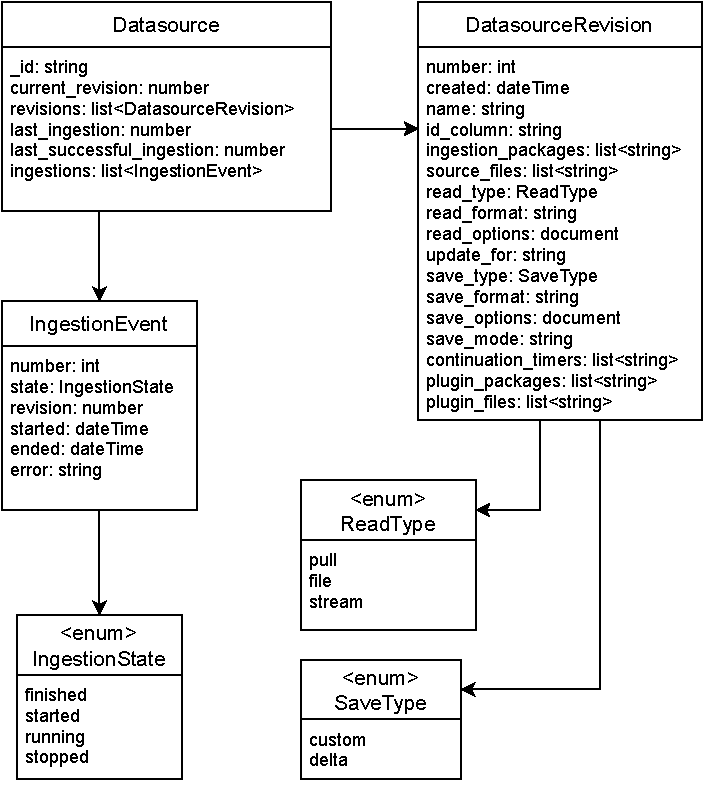
\includegraphics{Grafiken/ingestion-Datamodel.pdf}
    \caption{Datenmodell der Datenquelle}
    \label{fig:datasource_model}
\end{figure}

\subsection{Api-Server}

Da auch das Masterprojekt eine REST-Schnittstelle hat, bietet es sich an, diesen Server so zu erweitern, dass er als Api-Server für das neue System fungiert.
Um die neuen Endpunkte in die aktuelle Lösung zu integrieren, werden die existierenden Pfade, bis auf die zur Authentifizierung, nach "`/api/v1/"' verschoben und die neuen unter "`/api/v2/"' eingefügt.
Auf Grund der Tatsache, dass das neue System mit einem eigenen Datenmodell arbeitet, ist damit die Integration bereits abgehandelt, es muss nur darauf geachtet werden, die Funktionen der beiden Versionen zu trennen.
Die Endpunkte werden mit ihren Funktionen, wie in \fref{sec:arch} beschrieben, implementiert.

Bei der Erstellung und dem Aktualisieren von Datenquellen werden jedes mal eine neue Revision 
Dabei muss besonders darauf geachtet werden, dass bei jeder Änderung einer \verb|Datasource| eine neue \verb|DatasourceRevision| angelegt wird.
Die Quell- oder Plugindateien werden zentral im \textit{HDFS} jeweils einem Unterordner pro Datenquelle abgelegt.
So sind die Dateien von überall aus erreichbar und können auch bei replizierten oder verteilten Microservices verwendet werden.


\subsection{Ingestion-Server}



\subsection{Continuation-Server}

\section{Deltaerkennung}

\section{Datenversionierung}